%!TEX root = ../07-Electrical-Components.tex
\chapter{Current-Voltage Characteristics}

\begin{figure}[tbp]
	\centering
	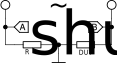
\includegraphics[width=.4\textwidth]{img/sch-iv-curve.pdf}
	\caption{Curve Tracer Schematic}
	\label{sch:curve}
\end{figure}

Current-Voltage Characteristics are recorded first in a quasi-static setup, later at higher frequencies.

\section{Setup}

To measure both current and voltage at the same time, the device under test and a shunt resistor $\mathrm{R_{shunt}}$ are connected in series to a function generator as shown in \autoref{sch:curve}.
The voltages across both the DUT and $\mathrm{R_{shunt}}$ are recorded by an oscilloscope.
As the oscilloscope and function generator are both referenced to earth ground, an isolation transformer is connected between the circuit and the function generator.

A sine wave with a frequency of \SI{20}{\hertz} is fed into the circuit.
The oscilloscope is set up in XY-mode with a record length of \SI{50}{\ms}, with the voltage across the DUT as X input and the current (calculated from the voltage across $\mathrm{R_{shunt}}$) as Y input.

For diodes, the forward voltage is approximated by drawing a tangent to the curve at the forward biased region and determining its intersection with the x axis.

\section{Evaluation (quasi static)}

\def\ivsubfigwidth{0.45\textwidth}
\def\ivgraphicswidth{1.1\textwidth}

\begin{figure}[tbp]
	\centering

	\begin{subfigure}{\ivsubfigwidth}
		\centering
		\includegraphics[width=\ivgraphicswidth]{data/plots/diodes-low-freq.pdf}
		\caption{Silicon and Germanium Diode}
		\label{plot:iv:si-ge-diode}
	\end{subfigure}
	\begin{subfigure}{\ivsubfigwidth}
		\centering
		\includegraphics[width=\ivgraphicswidth]{data/plots/z-diode-low-freq.pdf}
		\caption{Z-Diode}
		\label{plot:iv:z-diode}
	\end{subfigure}

% 	\caption{$I$-$V$ Curves of Diodes}
% 	\label{plot:iv:diodes}
% \end{figure}
%
% \begin{figure}[tbp]
% 	\centering
% 	\ContinuedFloat

	\begin{subfigure}{\ivsubfigwidth}
		\centering
		\includegraphics[width=\ivgraphicswidth]{data/plots/leds-low-freq.pdf}
		\caption{LEDs}
		\label{plot:iv:leds}
	\end{subfigure}
	\begin{subfigure}{\ivsubfigwidth}
		\centering
		\includegraphics[width=\ivgraphicswidth]{data/plots/photodiode-low-freq.pdf}
		\caption{Photodiode}
		\label{plot:iv:photodiode}
	\end{subfigure}

	\caption{$I$-$V$ Curves of Diodes}
	\label{plot:iv:diodes}
\end{figure}

\textbf{Silicon and Germanium Diodes} (\autoref{plot:iv:si-ge-diode})\\
Both show a characteristic diode curve, with no measurable reverse current.
The forward voltages are
\begin{equation*}
	U_\text{f, Si} = \SI{0.60}{\volt} \quad \text{and} \quad U_\text{f, Ge} = \SI{0.37}{\volt}.
\end{equation*}
The germanium diode has a lower forward voltage at low currents, but for currents higher than \SI{4}{\mA} the silicon diode's steeper slope makes it superior as a rectifier.

\textbf{Zener Diode} (\autoref{plot:iv:z-diode})\\
The zener diode behaves similarly to the silicon diode in the active region.
Unlike the other diodes, it also allows current to flow when it is reverse biased.
The reverse breakdown voltage is determined similarly to the forward voltage:
\begin{equation*}
	U_\text{f} = \SI{0.68}{\volt} \quad \text{and} \quad U_\text{r} = \SI{-4.1}{\volt}.
\end{equation*}
The reverse voltage is lower than the specified zener voltage of \SI{5.1}{\volt}, as the zener voltage is often specified at higher currents (\SI{\sim10}{\mA}).

In reverse breakdown mode, the zener diode has a low differential resistance (steep slope).
This means it can be used to stabilize the output voltage of power supplies that have a higer output impedance by connecting it reverse-biased in parallel to the load.

\textbf{LEDs} (\autoref{plot:iv:leds})\\
LEDs show similar characteristics to regular diodes, though they generally have a higher forward voltage (and they glow, I mean how fucking cool is that? \todo{remove humor}):
\begin{equation*}
	U_\text{f, red} = \SI{1.67}{\volt}, \quad U_\text{f, orange} = \SI{1.71}{\volt}, \quad U_\text{f, yellow} = \SI{1.80}{\volt}, \quad U_\text{f, green} = \SI{1.80}{\volt}
\end{equation*}

\textbf{Photodiode} (\autoref{plot:iv:photodiode})\\
The characteristic curve of a photodiode is similar to that of a normal diode in parallel with a light-dependent current source.
This means that the current is lowered (using the usual sign convention \todo{sounds stupid}) by a constant offset which is proportional to the light intensity.
Remarkably there is a region where current flows in the reverse direction, despite the positive bias voltage, thus energy can be extracted, photodiodes can be used as solar cells.
In most applications, photodiodes are used in the reverse bias region.

\begin{figure}[tbp]
	\centering

	\begin{subfigure}{\ivsubfigwidth}
		\centering
		\includegraphics[width=\ivgraphicswidth]{data/plots/ldr-low-freq.pdf}
		\caption{LDR}
		\label{plot:iv:ldr}
	\end{subfigure}
	\begin{subfigure}{\ivsubfigwidth}
		\centering
		\includegraphics[width=\ivgraphicswidth]{data/plots/varistor-low-freq.pdf}
		\caption{Varistor}
		\label{plot:iv:varistor}
	\end{subfigure}

	\caption{$I$-$V$ Curves of Resistors}	%sounds exciting, doesn't it?
	\label{plot:iv:boring}
\end{figure}

\textbf{LDR} (\autoref{plot:iv:ldr})\\
The characteristic curve of the LDR, like regular resistors, is a straight line through the origin.
Its slope is dependent on the light intensity, higher intensities resulting in a steeper slope.
The recorded diagram has a slope of \SI{1}{\mA\per\volt}, which corresponds to a resistance of \SI{1}{\kilo\ohm}.

\textbf{Varistor} (\autoref{plot:iv:varistor})\\
The characteristic curve of a varisor has a roughly symmetric diode-like bend.
The voltage drop is approximately \SI{\pm 5.5}{\volt} which is higher than the rating of \SI{3.3}{\volt} as it's designed to allow no current to flow at it's rated voltage.

It can be used to clamp the voltage across a sensitive component or an inductance by connecting it in parallel to the component/inductance.

\section{High Frequency Behavior}

The same test circuit is used with a sine wave of \SI{10}{\kHz}.

All tested components except for the LDR show hysterisis, due to stray capacitances, inductances and diode recovery times.

\begin{figure}[tbp]
	\centering

	\begin{subfigure}{\ivsubfigwidth}
		\centering
		\includegraphics[width=\ivgraphicswidth]{data/plots/diodes-hi-freq.pdf}
		\caption{Silicon and Germanium Diode}
		\label{plot:iv-hi:si-ge-diode}
	\end{subfigure}
	\begin{subfigure}{\ivsubfigwidth}
		\centering
		\includegraphics[width=\ivgraphicswidth]{data/plots/z-diode-hi-freq.pdf}
		\caption{Z-Diode}
		\label{plot:iv-hi:z-diode}
	\end{subfigure}

	\begin{subfigure}{\ivsubfigwidth}
		\centering
		\includegraphics[width=\ivgraphicswidth]{data/plots/led-hi-freq.pdf}
		\caption{red LED}
		\label{plot:iv-hi:leds}
	\end{subfigure}
	\begin{subfigure}{\ivsubfigwidth}
		\centering
		\includegraphics[width=\ivgraphicswidth]{data/plots/photodiode-hi-freq.pdf}
		\caption{Photodiode}
		\label{plot:iv-hi:photodiode}
	\end{subfigure}

	\begin{subfigure}{\ivsubfigwidth}
		\centering
		\includegraphics[width=\ivgraphicswidth]{data/plots/ldr-hi-freq.pdf}
		\caption{LDR}
		\label{plot:iv-hi:ldr}
	\end{subfigure}
	\begin{subfigure}{\ivsubfigwidth}
		\centering
		\includegraphics[width=\ivgraphicswidth]{data/plots/varistor-hi-freq.pdf}
		\caption{Varistor}
		\label{plot:iv-hi:varistor}
	\end{subfigure}

	\caption{$I$-$V$ Curves at \SI{10}{\kHz}}
	\label{plots:iv-hi}
\end{figure}
